            \section{Schärfen und Entfalten}
            (Gegenteil von Kapitel 5)
            \begin{enumerate}
                \item[Gegeben:] unscharfes Bild
                \item[Gesucht:] Version mit vielen erkennbaren Details
            \end{enumerate}

            \subsection{{Laplace-Schärfen}\index{Laplace-Schärfen}}
                Idee:

                \begin{center}
                \begin{tikzpicture}
                    \draw[dotted] (-0.5,0) node[left] {\small $u$:}-- (8.5,0);
                    \draw[scale=1,domain=-2:0,smooth,variable=\x,shift ={(2,0)}] plot ({\x},{(e^((-(\x)^2)/(0.2))}) -- (4,1) [scale=1,domain=0:2,smooth,variable=\x,shift ={(4,0)}] plot({\x},{(e^((-(\x)^2)/(0.2))});

                    \draw[dotted] (-0.5,-2) node[left] {\small $u''$:}-- (8.5,-2);
                    \draw[scale=1,domain=-1.5:1,smooth,variable=\x,shift ={(1.5,-2)}] plot ({\x},{-5*\x*(e^((-(\x)^2)/(0.05))}) -- (4,0) [scale=1,domain=-1:1.5,smooth,variable=\x,shift ={(5,0)}] plot({\x},{5*\x*(e^((-(\x)^2)/(0.05))});

                    \draw[dotted] (-0.5,-4) node[left] {\small $u - \tau u''$:}-- (8.5,-4);
                    \draw[scale=1,domain=-2:0,smooth,variable=\x,shift ={(2,-4)}] plot ({\x},{(e^((-(\x)^2)/(0.2))+4*(\x+0.5)*(e^((-(\x+0.5)^2)/(0.07))}) -- (4,1.056) [scale=1,domain=0:2,smooth,variable=\x,shift ={(4,0)}] plot({\x},{(e^((-(\x)^2)/(0.2))-4*(\x-0.5)*(e^((-(\x-0.5)^2)/(0.07))});

                \end{tikzpicture}
            \end{center}
            Zu sehen ist, dass durch die Subtraktion von $u''$, skaliert mit einem Faktor $\tau > 0$ die Kanten hervorgehoben werden.\\

            Hinweise zur Umsetzung:
            \begin{enumerate}[label=-]
                \item $u - \tau u''$ reskalieren (Kontrast-stretching) falls der Farbraum verlassen wird.
                \item $\tau$ kann auch sehr klein gewählt werden und der Vorgang dafür wiederholt iteriert werden.
                \item In 2D $\Delta$ statt 2. Ableitung
                \item Vorglätten: $u - \tau \C \Delta (G*u)$
            \end{enumerate}

            \subsection{Kantenverstärkende Diffusion}
                Verallgemeinerte Diffusionsgleichung: $\displaystyle \frac{\partial u}{\partial t} = div(M \nabla u)$.
                Idee: $M$ so wählen, so dass der Fluss:
                \begin{enumerate}[label=-]
                    \item Parallel zum Gradienten (d.h. durch die Kante verläuft): $\displaystyle \lambda_1=\frac{1}{1+\frac{\abs{\nabla u (\x)}^2}{\kappa^2}}$
                    \item senkrecht zu $\nabla u$ (entlang der Kante): $\lambda_2=1$
                \end{enumerate}

                $\Rightarrow M$ hat EW $\lambda_1$ zum EV $\displaystyle v_1= \frac{\nabla u}{\abs{\nabla u}}\srmatrix{\frac{\partial u}{\partial x}(\x)\\\frac{\partial u}{\partial y}(\x)}$ und EW $\lambda_2$ zum EV $\displaystyle v_2 = \frac{1}{\abs{\nabla u}} \srmatrix{-\frac{\partial u}{\partial y}(\x)\\\frac{\partial u}{\partial x}(\x)} \perp v_1$.\\
                $\displaystyle \Rightarrow M \C \underbrace{\mat{v_1 & v_2}}_{\small \text{orthogonale Matrix}} = \mat{\lambda_1 v_1 & \lambda_2 v_2} = \mat{v_1 & v_2} \mat{\lambda_1 & \ \\ \ & \lambda_2} \Rightarrow M^{-1} = M^T$\\
                $\Rightarrow M= \mat{v_1 & v_2} \mat{\lambda_1 & \ \\ \ & \lambda_2} \underbrace{\mat{v_1 & v_2}^T}_{=\mat{v_1^T \\ v_2^T}} = \frac{1}{\abs{\nabla u}^2} \mat{\lambda_1 \frac{\partial u}{\partial x}(\x)^2 + \lambda_2 \frac{\partial u}{\partial y}(\x)^2  & (\lambda_1 - \lambda_2)\frac{\partial u}{\partial x} \frac{\partial u}{\partial y}(\x)\\ (\lambda_1 - \lambda_2)\frac{\partial u}{\partial x} \frac{\partial u}{\partial y}(\x) & \lambda_2 \frac{\partial u}{\partial x}(\x)^2 + \lambda_1 \frac{\partial u}{\partial y}(\x)^2}$\\
                falls $\nabla u(\x) \neq 0$, sonst $M= \mat{1 & 0 \\ 0 & 1}$.

            \subsection{Entfaltung}\index{Entfaltung}
                \begin{center}
                    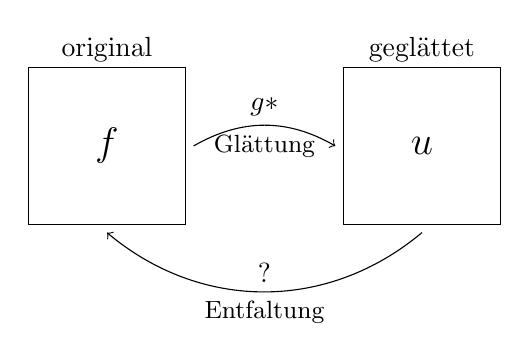
\begin{tikzpicture}
                        \draw (0,0) rectangle node[] {\Large $f$} node[above,yshift=27] {original} (2,2);
                        \draw (4,0) rectangle node[] {\Large $u$} node[above,yshift=27] {geglättet} (6,2);
                        \draw[] (2.1,1) edge[bend left,->]  node[above] {$g*$} node[below] {\small Glättung} (3.9,1);
                        \draw[] (1,-0.1) edge[bend right=40,<-]  node[above] {?} node[below] {\small Entfaltung} (5,-0.1);
                    \end{tikzpicture}
                \end{center}
                Das heißt: $u=f * g$, wobei $u, \ g$ gegeben sind und $f$ gesucht ist.\\
                Alternativ kann dies als die Invertierung des Faltungsoperator $f \mapsto g * f$ betrachtet werden.
                \begin{enumerate}[label = \alph*)]
                    \item Diskreter Fall: \begin{align*}
                                            & g*f=u\\
                                            &(g*f)(j)=u(j), \ j \in \Omega\\
                                            &\sum_k g(j-k)f(k)=u(j), \ j \in \Omega\\
                                            &\Rightarrow \Omega \times \Omega \text{ Gleichungsystem}
                                            \end{align*}
                        \begin{center}
                            \begin{tikzpicture}
                                \matrix [matrix of nodes, column sep=1mm, row sep=1mm,name=M,left delimiter={(},right delimiter={)}]
                                {
                                    {$g(0)$}& {$g(-1)$}& {}& {}& {}& {}& {}& {$g(-n)$}\\
                                    {$g(1)$}& {$g(0)$}& {$g(-1)$}& {}& {}& {}& {}& {}\\
                                    {}& {}& {}& {}& {}& {}& {}& {}\\
                                    {}& {}& {}& {}& {}& {}& {}& {}\\
                                    {}& {}& {}& {}& {}& {}& {}& {}\\
                                    {}& {}& {}& {}& {}& {}& {}& {}\\
                                    {}& {}& {}& {}& {}& {}& {}& {\phantom{g(-0)}}\\
                                    {}& {}& {}& {}& {}& {}& {}& {\phantom{g(0)}}\\
                                    {}& {}& {}& {}& {}& {}& {}& {\phantom{g(0)}}\\
                                    {$g(n)$}& {}& {}& {}& {}& {}& {}& {}\\
                                    };
                                    \draw[dotted] (M-2-2)--(M-8-8);
                                    \draw[dotted] (M-2-1)--(M-9-8);
                                    \draw[dotted] (M-2-3)--(M-7-8);
                                    \draw (M-1-1) node[left,xshift =-23] {$j=0$};
                                    \draw (M-2-1) node[left,xshift =-23] {$j=1$};
                                    \draw (M-10-1) node[left,xshift =-23] {$j=n$};
                                    \draw (M-1-1) node[yshift =23] {$k=0$};
                                    \draw (M-1-2) node[yshift =23] {$k=1$};
                                    \draw (M-1-8) node[yshift =23] {$k=n$};
                                    \draw[decorate,decoration={brace,amplitude=4pt,mirror}] (-3.3,-3) -- node[below] {\textbf{Toeplitz-Matrix}\index{Toeplitz-Matrix}} (3.5,-3);
                                    \matrix [matrix of nodes, column sep=1mm, row sep=1mm,name=N,left delimiter={(},right delimiter={)},shift={(5,0)}]
                                    {
                                    {$f(0)$}\\
                                    {$f(1)$}\\
                                    {}\\
                                    {}\\
                                    {}\\
                                    {}\\
                                    {}\\
                                    {}\\
                                    {}\\
                                    {}\\
                                    {}\\
                                    {}\\
                                    {$f(n)$}\\
                                    };
                                \draw[dotted] (N-2-1) -- (N-13-1);
                                \draw (6.9,0) node[] {\Large $=$};
                                \matrix [matrix of nodes, column sep=1mm, row sep=1mm,name=O,left delimiter={(},right delimiter={)},shift={(8.5,0)}]
                                {
                                    {$u(0)$}\\
                                    {$u(1)$}\\
                                    {}\\
                                    {}\\
                                    {}\\
                                    {}\\
                                    {}\\
                                    {}\\
                                    {}\\
                                    {}\\
                                    {}\\
                                    {}\\
                                    {$u(n)$}\\
                                    };
                                \draw[dotted] (O-2-1) -- (O-13-1);
                            \end{tikzpicture}
                        \end{center}
                        \item Kontinuierlicher Fall: \begin{align*}
                                                        &(g*f)(x)=u(x),\ x \in \Omega\\
                                                        &\int_\R g(x-y) f(y) dy = u(x), \ x \in \Omega\\
                                                        &\text{Integralgleichung für die gesuchte Funktion $f$}
                                                        \end{align*}
                        $\Rightarrow$ Kontinuierliche Matrix:

                        \begin{center}
                            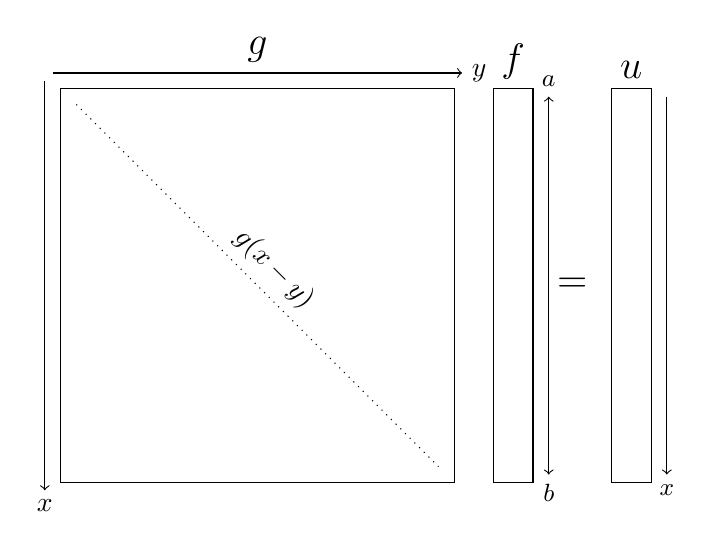
\begin{tikzpicture}
                                \draw (0,0) rectangle (5,5);
                                \draw[->] (-0.2,5.1) -- (-0.2,-0.1) node[below] {$x$};
                                \draw[->] (-0.1,5.2) -- (5.1,5.2) node[right] {$y$};
                                \draw[] (2.5,5.5) node {\Large $g$};
                                \draw[dotted] (0.2,4.8) -- node[sloped,above] {$g(x-y)$} (4.8,0.2);
                                \draw (5.5,5) node[above,xshift=7] {\Large $f$} rectangle (6,0);
                                \draw[<->] (6.2,4.9) node[above] {\small $a$} -- (6.2,0.1)  node[below] {\small $b$};
                                \draw (6.5,2.5) node[] {\Large $=$};
                                \draw (7,5) node[above,xshift=7] {\Large $u$} rectangle (7.5,0);
                                \draw[->] (7.7,4.9) -- (7.7,0.1) node[below] {\small $x$};
                            \end{tikzpicture}
                        \end{center}
                        Wobei $[a,b]$ die das Definitionsgebiet von $f$ ist.
                        Diese Problem is jedoch schlecht gestellt, da der Operator kompakt ist. ($\nearrow$ Datei im Studip)
                \end{enumerate}

                Wir versuchen es trotzdem zu lösen:
                \begin{align*}
                    g*f&=u & &|\cdot \F\\
                    \F(g * f)&= \F u \\
                    (2 \pi)^\frac{d}{2}(\F g)\cdot (\F f)&= \F u & &| \div (2 \pi)^\frac{d}{2}(\F g)\\
                    \F f &= \frac{\F u}{(2 \pi)^\frac{d}{2} \F g} & &| \F^{-1}
                \end{align*}
                Und erhalten:
                \begin{equation}
                    f= (2 \pi)^\frac{d}{2} \F^{-1}\left(\frac{\F u}{\F g}\right)
                \end{equation}
                Dieses kann jedoch zu Problemen führen, da etwa $g \approx 0$ werden kann.
                Je glatter $g$ ist, desto stärker klingt $(\F g)(z)$ ab für $z \to \infty$.\\
                \ \\
                Anders betrachtet:\\
                Wenn $\abs{\hat g(z)}$ für hohe Frequenzen klein ist, dann ist:
                \[A:f \mapsto g +f\]
                ein Tiefpassfilter. Nimmt man nun eine Funktion $h$ mit hoher Frequenz und großer Amplitude, dann gilt:
                \[A(f + h) = Af + \underbrace{Ah}_{\approx 0} \approx Af\]

                \underline{Problembehebung:}
                \begin{enumerate}[label = \arabic*. Ansatz:]
                    \item \ \\
                    \begin{minipage}[c]{0.55\textwidth}
                        \begin{center}
                            Approximiere die Funktion $\frac{1}{x}$ durch\\
                            \[R_\alpha = \begin{cases}
                                \frac{1}{x}, & \abs{x} > \alpha\\
                                \frac{1}{\alpha}, & x \in [0,\alpha]\\
                                \frac{1}{-\alpha}, & x \in [-\alpha,0]
                            \end{cases}\]
                            wobei $\alpha > 0$.
                        \end{center}
                        und ersetze $\displaystyle f=(2 \pi)^\frac{d}{2} \F^{-1}\left(\frac{\hat u (z)}{\hat g(z)}\right)$ durch:\\
                        \[f=(2 \pi)^\frac{d}{2} \F^{-1}\left(\hat u (z) R_\alpha(\hat g(z)) \right)\]
                        und lasse $\alpha \to 0$.
                    \end{minipage}
                    %\hfill\vrule\hfill
                    \begin{minipage}[c]{0.4\textwidth}
                        \begin{center}
                            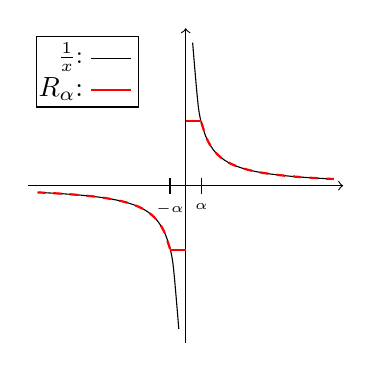
\begin{tikzpicture}
                                \draw[->] (-2,0) -- (2,0);
                                \draw[<-] (0,2) -- (0,-2);
                                \draw[scale=0.4,domain=0.22:4.7,smooth,variable=\x,shift ={(0,0)}] plot ({\x},{1/\x});
                                \draw[scale=0.4,domain=-0.22:-4.7,smooth,variable=\x,shift ={(0,0)}] plot ({\x},{1/\x});
                                \draw[scale=0.4,domain=0.5:4.7,smooth,variable=\x,shift ={(0,0)},dashed,red,thick] plot ({\x},{1/\x});
                                \draw[scale=0.4,domain=-0.5:-4.7,smooth,variable=\x,shift ={(0,0)},dashed,red,thick] plot ({\x},{1/\x});
                                \draw (0.2,0.1) -- (0.2,-0.1) node[below] {\tiny $\alpha$};
                                \draw (-0.2,0.1) -- (-0.2,-0.1) node[below] {\tiny $-\alpha$};
                                \draw[color=red,thick] (0,0.81818) -- (0.2,0.81818);
                                \draw[color=red,thick] (0,-0.81818) -- (-0.2,-0.81818);
                                \draw (-1.9,1.9) rectangle node[align=right,left,xshift = 2] {\small $\frac{1}{x}$:\\$R_\alpha$:} (-0.6,1);
                                \draw (-1.2,1.62)--(-0.7,1.62);
                                \draw[thick,red] (-1.2,1.22)--(-0.7,1.22);
                            \end{tikzpicture}
                        \end{center}
                    \end{minipage}
                    \item Variationsrechnung:
                        \begin{enumerate}[label = \arabic*. Wunsch:]
                            \item $g *f \approx u$
                            \item $\norm{f}_2$ klein
                        \end{enumerate}
                        Minimiere nun:
                        \[\Rightarrow J(f)  \coloneqq  \norm{g * f - u}_2^2 + \lambda \norm{f}_2^2 \to min\]
                        \[\iff \int_{\R^d} ((g*f)(x) - u(x))^2 + \lambda f(x)^2 dx \to min\]
                        über die Wahl von $f \in U \coloneqq  L^2(\R^d)$.\\
                        Idee: $\F$ anwenden $\Rightarrow *$ wird zu $\C$ \underline{und} $\norm{\C}_2$ bleibt unverändert.
                        \begin{align*}
                            \Rightarrow J(f)&=\norm{g*f-u}_2^2 + \lambda\norm{f}_2^2\\
                            &=||\widehat{g*f-u}||_2^2 + \lambda ||\hat f||_2^2\\
                            &=||(2 \pi)^\frac{d}{2} \hat g \hat f -\hat u||_2^2 + \lambda||\hat f||_2^2\\
                            &=\int_{\R^d}\left[ \left|(2 \pi)^\frac{d}{2} \hat g(z) \hat f(z) - \hat u(z)\right|^2 + \lambda |\hat f(z)|^2 \right] dz \overset{f \in U}{\longrightarrow} min
                        \end{align*}
                    Strategie: Integral für jedes einzelne $z$ minimieren. Daraus erhalten wir ein optimales $\hat f$ und somit auch ein optimales $f$.\\
                    Also minimiere für jedes $z \in \R^d$
                    \[I(t) \coloneqq |(2 \pi)^\frac{d}{2} \hat g(z)t - \hat u(z)|^2 + \lambda |t|^2 \overset{t \in \mathbb C}{\longrightarrow}min\]
                    Später setzen wir $\hat f(z) \coloneqq t_{min}$, nun zur Minimierung:
                    \begin{align*}
                        I(t)&=((2 \pi)^\frac{d}{2} \hat g(z) t - \hat u(z))((2 \pi)^\frac{d}{2} \ \overline{\hat g(z)} \ \overline t -\overline{\hat u (z)}) + \lambda t \overline t\\
                        &=(2 \pi)^\frac{d}{2} \hat g(z) \ \overline{\hat g(z)} \ t \ \overline t + \lambda t \overline t - (2 \pi)^\frac{d}{2} (\hat g(z) \ \overline{\hat u(z)} \ t + \overline{\hat g(z)} \ \hat u(z) \ \overline{t}) + \hat u(z) \ \overline{\hat u(z)}\\
                        &=((2 \pi)^\frac{d}{2} |\hat g(z)|^2 + \lambda)|t|^2 - (2 \pi)^\frac{d}{2} (2 \C Re(\underbrace{\hat g(z) \ \overline{\hat u(z)}t}_{\circledast})) + |\hat u(z)|^2 \overset{t \in \mathbb C}{\longrightarrow} min\\
                    \end{align*}
                    Das Argument (Winkel) taucht nur in $\circledast$ auf\\
                    \begin{align*}
                        &\Rightarrow \text{So wählen, das $\circledast$ auf die positive reele Achse fällt}\\
                        &\Rightarrow 0=arg(\circledast)= arg(\hat g(z) \ \overline{\hat u(z)}) + arg(t)\\
                        &\Rightarrow arg(t)=-arg(\hat g(z) \ \overline{\hat u(z)})=arg(\overline{\hat g(z)} \ \hat u(z))\\
                        &\Rightarrow I(t) = ((2\pi)^\frac{d}{2} |\hat g(z)|^2 + \lambda)|t|^2 - (2\pi)^\frac{d}{2} 2 \C |\overline{\hat g(z)} \ \hat u(z)| \ |t| + |\hat u (z)|^2 \overset{|t| \in \R}{\longrightarrow}min
                    \end{align*}
                    Dieses ist nun ein Polynom in $|t|$, sodass das Minimum einfach bestimmt werden kann.\\
                    \begin{align*}
                        &0=\frac{d}{d|t|}...=2\C((2\pi)^\frac{d}{2}|\hat g(z)|^2 + \lambda)|t| - (2\pi)^\frac{d}{2} \C 2 \C |\overline{\hat g(z)} \ \hat u(z)|\\
                        &\Rightarrow |t| = \frac{(2\pi)^\frac{d}{2} \C 2 \C |\overline{\hat g(z)} \ \hat u(z)|}{2\C((2\pi)^\frac{d}{2}|\hat g(z)|^2 + \lambda)} = \frac{(2\pi)^\frac{d}{2}\C |\overline{\hat g(z)} \ \hat u(z)|}{(2\pi)^\frac{d}{2}|\hat g(z)|^2 + \lambda} \text{ und } arg(u)=arg(\overline{\hat g(z)} \ \hat u(z))\\
                        &\Rightarrow t =  \frac{(2\pi)^\frac{d}{2} \ \overline{\hat g(z)} \ \hat u(z)}{(2\pi)^\frac{d}{2}|\hat g(z)|^2 + \lambda}=:\hat f(z)
                    \end{align*}
                    Wegen
                    \[\hat f(z) = (2\pi)^\frac{d}{2} \frac{\overline{\hat g(z)}}{(2\pi)^\frac{d}{2}|\hat g(z)|^2 + \lambda} \hat u(z)\]
                    gilt
                    \begin{equation}
                        f(z) = \F^{-1}\left( \frac{\overline{\hat g(z)}}{(2\pi)^\frac{d}{2}|\hat g(z)|^2 + \lambda} \right) * u
                    \end{equation}
                    Dieses Verfahren wird \textbf{$L^2$ deblurring}\index{$L^2$ deblurring} genannt.
                    Es gibt auch einen alternativen, algebraischen Zugang:

                    \[I(f) = \norm{g*f-u}_2^2 + \lambda \norm{f}_2^2 \overset{f}{\to} min\]
                    \[\iff \norm{\mat{g*f-u\\ \sqrt{\lambda} f}} \overset{f}{\to} min\]
                    \[\iff \norm{\mat{Af \\ \sqrt{\lambda}f} - \mat{u\\0}} = \norm{\mat{A \\ \sqrt{\lambda}}f - \mat{u\\0}} \overset{f}{\to} min \quad (A= f \mapsto g*f)\]
                    $\Rightarrow$ lineares Ausgleichsproblem.
                    \[\Rightarrow \mat{A^* &\sqrt{\lambda} I^*} \mat{A \\ \sqrt{\lambda}I}f = \mat{A^* & \sqrt{\lambda}I} \mat{u \\ 0} \quad \text{(Normalengleichung)}\]
                    \[\Rightarrow \mat{A^*A + \abs{\lambda}I}f=A^*u\]
                    \[\Rightarrow f= \mat{A^*A + \abs{\lambda}I}^{-1}A^*u\]
                    Die Inverse existiert, da $-\abs{\lambda}$ nicht im Spektrum von $A^*A$ sein kann, denn das Spektrum von $A^*A$ ist positiv und reel.
                    \item noch einmal Variationsrechnung, diesmal mit anderen Wünschen
                    \begin{enumerate}[label = \arabic*. Wunsch:]
                        \item $g *f \approx u$
                        \item $\norm{\nabla f}$ klein
                    \end{enumerate}
                    Nach analoger Rechnung wie oben erhält man:
                    \begin{equation}
                        f=\F \left( \frac{\overline{\hat g(z)}}{(2\pi)^\frac{d}{2} \ |\hat g(z)|^2 + \lambda |z|^2} \right) * u
                    \end{equation}
                    $\Rightarrow$ Dämpfung höher wenn Frequenz höher.\\
                    Dieses Verfahren nennt sich \textbf{$H^1$ deblurring}\index{$H^1$ deblurring}.
                \end{enumerate}

